


\documentclass[11pt,a4paper,uplatex,draft]{ujarticle} 
\usepackage{bm}
\usepackage{amsmath}
\usepackage{comment}
\usepackage{amsthm}       
\usepackage{multicol}
\usepackage{subcaption}
\usepackage{setspace}
\usepackage{MnSymbol}
\usepackage{listings,jvlisting}
\usepackage{enumerate}
\usepackage{braket}
\usepackage[version=3]{mhchem} % Package for chemical equation typesetting
\usepackage{siunitx} % Provides the \SI{}{} and \si{} command for typesetting SI units
\usepackage[dvipdfmx]{graphicx, hyperref}%,hyperref % Required for the inclusion of images
\usepackage{pxjahyper}%, Required to fix garbled text
\usepackage[square,sort,comma,numbers]{natbib} % Required to change bibliography style to APA

% \setlength\parindent{0pt} % Removes all indentation from paragraphs
\hypersetup{colorlinks=true, linkcolor=black} %delete red lines 
\makeatletter
\newcommand{\figcaption}[1]{\def\@captype{figure}\caption{#1}}
\newcommand{\tblcaption}[1]{\def\@captype{table}\caption{#1}}
\makeatother

%----------------------------------------------------------------------------------------
%	DOCUMENT INFORMATION
%----------------------------------------------------------------------------------------

%ここからソースコードの表示に関する設定
\lstset{
  basicstyle={\ttfamily},
  identifierstyle={\small},
  commentstyle={\smallitshape},
  keywordstyle={\small\bfseries},
  ndkeywordstyle={\small},
  stringstyle={\small\ttfamily},
  frame={tb},
  breaklines=true,
  columns=[l]{fullflexible},
  numbers=left,
  xrightmargin=0zw,
  xleftmargin=3zw,
  numberstyle={\scriptsize},
  stepnumber=1,
  numbersep=1zw,
  lineskip=-0.5ex
}
\hypersetup{citecolor=black}
\usepackage[top=30truemm,bottom=30truemm,left=25truemm,right=25truemm]{geometry}
% 全体のページ設定
% ページ番号をフッタにふる
% \pagestyle{plain}
\makeatletter
 
\def\@thesis{2023年度 卒業論文中間報告書}
\def\teacher#1{\def\@teacher{#1}}
\def\department#1{\def\@department{#1}}
\def\id#1{\def\@id{#1}}
 
\def\@maketitle{
\begin{center}
{\Large \@thesis \par} %修士論文と記載される部分
\vspace{30mm}
{\Huge\bf \@title \par}% 論文のタイトル部分
\vspace{30mm}
{\Large \@date 提出\par} % 提出年月日部分
\vspace{20mm}
{\Large 指導教員 \@teacher \par} % 指導教員部分
\vspace{10mm}
{\Large \@department \par} % 所属部分
\vspace{10mm}
{\Large 学生証番号 \@id \par} % 学籍番号部分
\vspace{15mm}
{\Large \@author}% 氏名
\end{center}
%\par\vskip 1.5em
}

\makeatother

\title{複素ニューラルネットワークを用いた\\円偏波地中レーダシステム}
\teacher{廣瀬 明 教授\\
		\qquad \qquad \qquad 夏秋 嶺 准教授}
\date{2023年 9月29日}
\department{東京大学 工学部 電気電子工学科}
\id{03-220524}
\author{渡辺 裕貴}
\begin{document}

\maketitle
\newpage
\tableofcontents
\newpage
\section{序論}

  地中レーダによる計測は、地中に向けて電磁波を放射し、地中の埋設物から散乱された電磁波を受信することで、非破壊的に地中埋設物を探査する方法
  である。地雷検出や遺跡調査、インフラ整備のためのパイプの検知など多くの分野に応用されている\cite{landmine_example}\cite{remains_example}。

  地中レーダでは、送信用と受信用のアンテナのそれぞれについて2つの偏頗状態(典型的には水平偏波と垂直偏波)の2種類のアンテナを用意し、2$\times$2
  の散乱行列を取得する場合(フルポラリメトリック)と、送信あるいは受信用のアンテナのいずれか、もしくは両方について、一つの偏波状態の電磁波
  のみを扱う場合がある。フルポラリメトリックの場合では、対象物の散乱の特性について詳細な情報が得られる一方で、計測に時間がかかり、
  送受信アンテナの偏波を切り替える必要があるために計測システムが大きくなるデメリットがある。

  地中レーダに直線偏波を用いる場合では、散乱の特性が対象物の方向に依存しやすい。
  例えば、パイプのような直線状の対象物を直線偏波でセンシングする場合を
  考えると、電界の方向と対象物が平行になった時に大きな散乱が起こる一方で、電界の方向と対象物が垂直である場合には、散乱が非常に小さくなる。
  そのため、地中レーダに直線偏波を用いる場合には対象物の方向にかかわらず十分な散乱特性を得られるようフルポラリメトリック
  のシステムがよく用いられる。
  
  一方で、地中レーダに円偏波を用いる場合には、円偏波の次のような性質から、フルポラリメトリックでないシステムであっても地中レーダシステムとして十分な機能を持つ可能性がある。
  一つは対象物からの散乱が対象物の方向に依存しにくいこと、もう一つは完全導体における円偏波の散乱の場合に、散乱の前後で円偏波における電界の旋回方向が反転する
  ことである。
  後者の性質に関しては、導体の計測対象からの1回の散乱波を受信したい場合には、散乱の前後で電磁波の進行方向が逆転することを考慮し、受信アンテナを受信偏波の旋回方向に合わせた
  円偏波アンテナとすることで、所望の散乱波を選択的に受信できる。

  また、地中レーダデータに対してニューラルネットワークを用いた適応的な解析が行われてきており、その有効性が示されつつある\cite{landmine_CNN}\cite{hidden_Markov}。

  しかし、円偏波地中レーダでどのようにニューラルネットワークを構成知ると効果的であるかは議論されてこなかった。
\section{関連研究}

  \subsection{地中レーダにおけるデータの処理}

    地中レーダ技術の原理は、送信アンテナから地表に向かってパルス波を放射し、地中の埋設物からの散乱波を受信することで、地中の埋設物についての情報を
    得るものである。パルス波が放射されてからそれが対象物により散乱され受信アンテナに戻ってくるまでの時間の情報と、地中における電磁波の伝搬速度から
    地中における対象物の位置を推定することが可能である。パルス型の地中レーダは、実際にパルスを地表に向かって照射することで動作する。

    パルス型の他に、地中レーダとして連続波周波数掃引型地中レーダ(Stepped-Frequency Continuous Wave Ground Penetrating Radar, SFCW GPR)
    が用いられることがある。SFCW GPRでは、実際にパルス波を放射するのではなく、単一周波数成分のみをもつ電磁波を広帯域にわたって周波数を刻んで掃引して放射し、
    得られた受信波の振幅および位相を逆フーリエ変換することで、パルス波を放射した場合の散乱特性を再現する\cite{stepped_frequency_continuous_wave}。

    図\ref{fig:GPR_raw_data}は、Kido et. al[2011]により行われた実験\cite{STFW_Kido}における、地中パイプの(a) パルス型GPR (b) SFCW GPR を用いた
    可視化画像である。(a)は中心周波数$500\mathrm{MHz}$のパルスが用いられており、(b)は$50\mathrm{MHz}$から$1.5\mathrm{GHz}$を$10.66\mathrm{MHz}$
    間隔で掃引したSFCW GPRを用いた結果である。
    いずれの場合においても、地中のパイプからの放射に由来するとみられる双曲線関数形の信号強度の縞が可視化されており、これは地中レーダにおける典型的な
    信号である。

    一般に、地中レーダの生データでは、土壌の不均一性による散乱が起こり、目標の信号である対象物からの反射が土壌での散乱による信号に埋もれてしまうことが問題である
    \cite{prestack_migration}。これを解決するために、マイグレーションという手法が用いられることがある。マイグレーションは、対象物からの反射波を反射
    体位置から放射されたものと考え、複数の受信点から反射波の観測を考慮することで、より精確なイメージングを図る方法である\cite{gpr_migration}。

    \begin{figure}[htbp]
      \centering
      \begin{minipage}[b]{0.45\hsize}
        \centering
        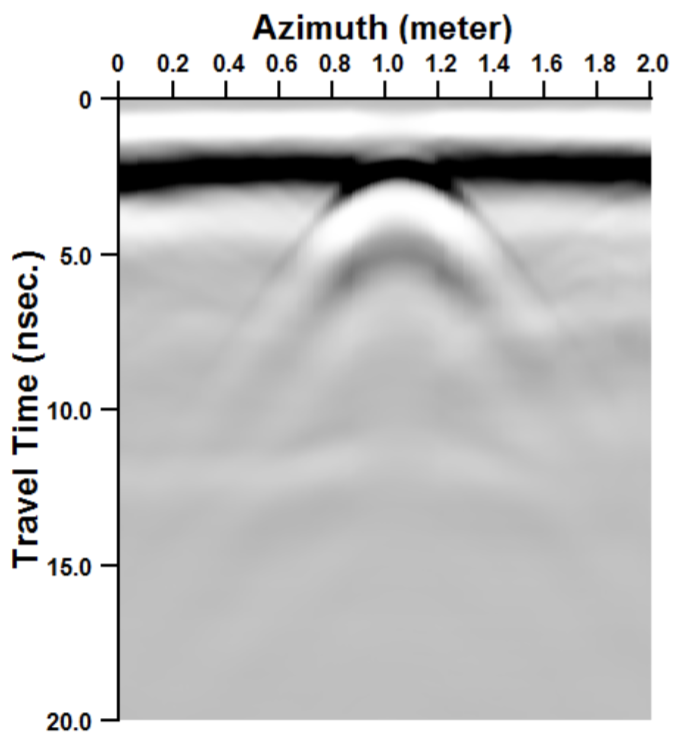
\includegraphics[keepaspectratio, width=70mm]{Images/SFCW_Kido.png}
        \subcaption{STFW}\label{SFCW_Kido}
      \end{minipage}
      \begin{minipage}[b]{0.45\hsize}
        \centering
        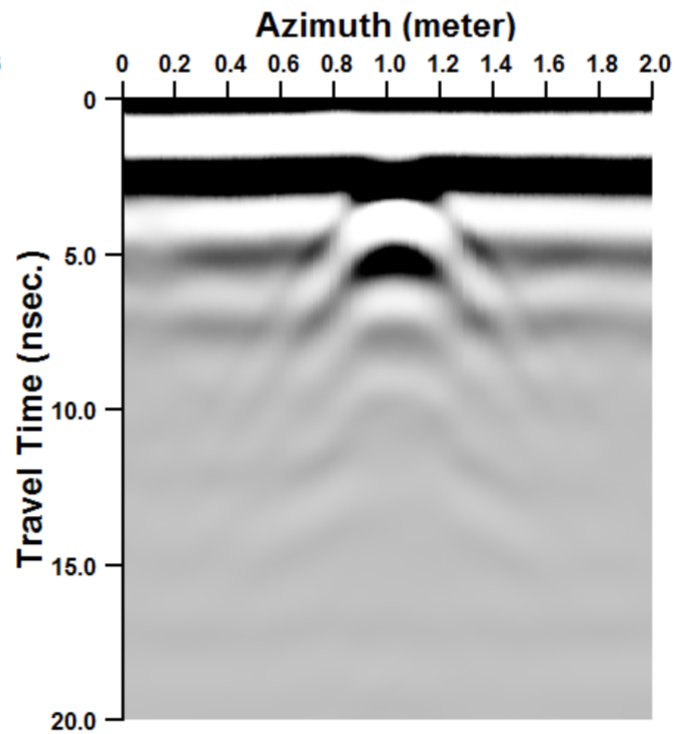
\includegraphics[keepaspectratio, width=70mm]{Images/pulse_Kido.png}
        \subcaption{パルス型}\label{pulse_Kido}
      \end{minipage}
      \caption{GPRシステムにより可視化されたパイプ\cite{STFW_Kido}}\label{fig:GPR_raw_data}
    \end{figure}

  \subsection{複素ニューラルネットワーク}

    ニューラルネットワークとは、TODO: setsumei
    複素ニューラルネットワークは、ニューラルネットワークのうち、特に入出力やパラメータが複素数であるものをいう。
    複素数は振幅のみでなく位相の情報を含むため、特に電磁波などの波動を扱うときに有効である\cite{CVNN}。

    具体的なニューラルネットワークにおける出力の方法は次の通りである。第$x$層の入力を$\bm{x}$、出力を$\bm{y}$、荷重を$\bm{W}$、バイアスを$b$、活性化関数を$f$とすると、出力$\bm{x_1}$は
    \begin{equation}
      \bm{y} = f(\bm{W}\bm{x})
    \end{equation}
    のように決定される。
    ここで、$f(x)$は活性化関数であり、ベクトルに作用させた場合は各要素に対して作用するものとする。複素数に対する活性化関数としては、例えば、
    \begin{equation}\label{activation_function}
      f(x = Ae^{i\theta}) = \tanh(A)e^{i\theta}
    \end{equation}
    のように、振幅のみを非線形化し、位相はそのままにするものが用いられる。階層型のニューラルネットワークの場合は、
    第$l$層の入力$\bm{x}_l$に対する出力$\bm{y}_l$を次の層の入力$\bm{x}_{l+1}$として用い、これを繰り返すことで、最終的な出力層の出力を得る。

    ニューラルネットワークにおける学習の際に正解となる信号(教師信号)が与えられる学習を教師あり学習という。教師信号と出力の誤差を出力層からより前段の層に向けて逆向きに伝搬させ
    層間の荷重の更新を行う誤差逆伝搬法が代表的である。
    実数ニューラルネットワークにおける学習方法としては
    \begin{equation}
      w_{nm} \leftarrow w_{nm} - lr \frac{\partial E}{\partial w_{nm}}
    \end{equation}
    のように、誤差関数の勾配を用いて荷重の更新を行う。ここで、$lr$は学習率、$E$は誤差関数である。

    複素数に対する誤差関数としては、例えば、
    \begin{equation}\label{error_function}
      \begin{split}
      E(\bm{t}, \bm{y})  & = \frac{1}{2}|\bm{t} - \bm{y}|^2\\
      & = \frac{1}{2}\sum_{i=1}^{N}|\bm{t}_i - \bm{y}_i|^2
      \end{split}
    \end{equation}
    が用いられる。ここで、$\bm{t}$は教師信号、$\bm{y}$は出力信号である。
    複素ニューラルネットワークにおける学習においては、
    活性化関数として式\ref{activation_function}を、誤差関数として式\ref{error_function}を用いた場合、
    \begin{equation}
      \label{eq:update_a}
      \begin{split}
        |w_{nm}| \leftarrow |w_{nm}| - lr^\mathrm{a} & \biggl( (1-|x_{l\,n}^2|)(|x_{l\, n}| - |t_{l\, n}| \cos (\angle x_{l\, n} - \angle t_{l\, n}))|x_{l-1\, m}| \cos \theta^{\mathrm{rot}}_{nm}  \\
                        & - |x_{l\, n}| |t_{l\, n}| \sin (\angle x_{l\, n} - \angle t_{l\, n}) \frac{|x_{l-1\, m}|}{|u_{l\, n}|} \sin \theta^{\mathrm{rot}}_{nm} \biggr)
      \end{split}
    \end{equation}
    \begin{equation}
      \label{eq:update_p}
      \begin{split}
        \angle w_{nm} \leftarrow \angle w_{nm} - lr^\mathrm{p} & \bigg( (1-|x_{l\,n}^2|)(|x_{l\, n}| - |t_{l\, n}| \cos (\angle x_{l\, n} - \angle t_{l\, n}))|x_{l-1\, m}| \sin \theta^{\mathrm{rot}}_{nm} \\
                        &  + |x_{l\, n}| |t_{l\, n}| \sin (\angle x_{l\, n} - \angle t_{l\, n}) \frac{|x_{l-1\, m}|}{|u_{l\, n}|} \cos \theta^{\mathrm{rot}}_{nm} \bigg)
      \end{split}
    \end{equation}
    \begin{equation}
      \label{eq:rot}
        \theta^{\mathrm{rot}}_{nm} = \angle x_{l\, n} - \angle x_{l-1\, m} -\angle w_{nm}
    \end{equation}

    に従って振幅、位相ごとに荷重の更新を行うことで、誤差関数を小さくする方向に学習を進めることができる。\cite{CVNN}
    TODO:検討 正しい?どのくらい書く?変数の意味は?



\section{複素ニューラルネットワークを用いた円偏波地中レーダシステム}

  % \subsection{システム設計の目的}
  
  \subsection{システムの特徴}
    
    提案システムは、送受信アンテナ、これに接続されたベクトルネットワークアナライザ、XYステージからなる計測システムと、複素ニューラルネットワークを用いた
    解析システムにより構成される。
    % 本システムにおけるデータ解析は、
    % 対象物の向きや形状などの幾何構造や、対象物の存在する座標などの特徴量について、従来的な方法のように対象物からの散乱の様子を信号処理的に可視化することで
    % 推定するのではなく、複素ニューラルネットワークを用いて適応的に抽出することを目標としている。
    従来的な方法では、対象物からの散乱の様子を信号処理的に推定するものである。それに対し、本システムにおけるデータ解析の目標は、対象物の向きや形状などの幾何構造や、
    対象物の存在する座標などの特徴量について、複素ニューラルネットワークを用いて適応的に抽出することである。

  \subsection{計測システムの構成}

    計測システムの概要図を図\ref{fig:XYstage_configuration}に示す。
    文献\cite{absorbing_material}に倣い、送受信アンテナ部分は、図\ref{fig:absorbing_material}に示すようにアンテナとバランを
    電磁波吸収体からなる中空円筒で覆う。これにより、所望の放射方向である地表面方向以外へ電磁波が放射されるのを抑制する。送受信アンテナ部分は、それぞれベクトルネットワーク
    アナライザの異なるポートに同軸ケーブル、バランを通じて接続されている。アンテナ部分は、送受信アンテナの相対的な位置が固定された状態で、XYステージにより
    実験用土槽上の任意の座標に動かすことができる。
    計測システムは、XYステージによる地表面の走査を、設定した各周波数で繰り返すことで、XYステージ上の2次元の座標と周波数ごとに、振幅と位相の情報をもつ複素数のデータ
    が得られるように構成する。

    \begin{figure}[hbtp]
      \centering
      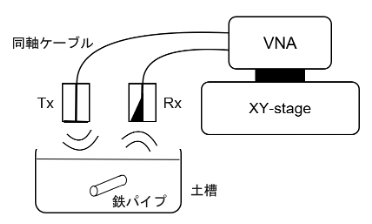
\includegraphics[keepaspectratio, width=130mm]{Images/XYstage_configuration.png}
      \caption{計測システムの概略図}\label{fig:XYstage_configuration}
    \end{figure}

    \begin{figure}[hbtp]
      \centering
      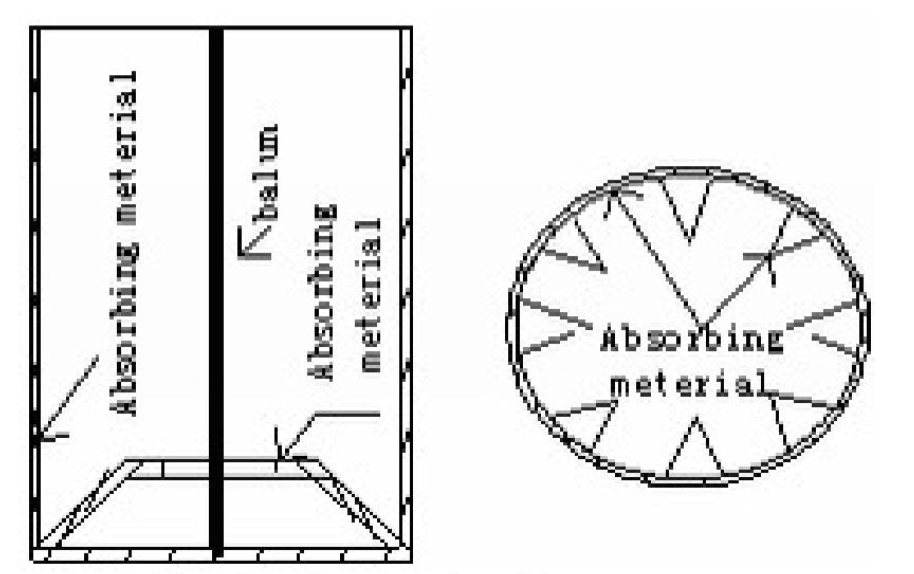
\includegraphics[keepaspectratio, width=130mm]{Images/absorbing_material.png}
      \caption{電波吸収体で覆われたアンテナシステムの構造\cite{absorbing_material}}\label{fig:absorbing_material}
    \end{figure}

  \newpage

  \subsection{複素ニューラルネットワークを用いた解析システム}

    計測システムにより得られた複素数データを、複素ニューラルネットワークを用いて解析する。具体的に用いる複素ニューラルネットワークは未実装であるが、
    その展望については\ref{CVNN_plan}節で述べる。

\section{実験}

  \subsection{円偏波地中レーダに用いるアンテナの設計}

  本研究では、地中レーダとして円偏波アンテナを用いる。地中レーダに用いられるアンテナとしては、スパイラルアンテナを用いる。実際の計測に際しては、
  ベクトルネットワークアナライザにアンテナを接続して用いる。VNA からの給電の際には、同軸ケーブルを通じてアンテナに給電するため、同軸ケーブルと
  アンテナの間にバランを設ける。このバランは、不平衡-平衡の変換を行うだけでなく、特性インピーダンスが$50\Omega$である同軸ケーブルと、一般にこれと
  異なる入力インピーダンス特性を持つアンテナ間のインピーダンスの整合も兼ねる。そのため、アンテナの入力インピーダンス特性を調べた上で、適切な
  インピーダンス変換を行うことができるように設計する必要がある。

  実際に設計したアンテナおよびバランを、それぞれ図\ref{fig:spiral_antenna_configuration}および図\ref{fig:taper_balun_configuration}に示す。
  設計には、有限要素法による高周波電磁界シミュレーションソフトウェアであるAnsys HFSSを用いた。

  アンテナはスパイラルバランとして設計し、導体ライン幅は$3.0\mathrm{mm}$、導体ライン間のギャップは$4.1\mathrm{mm}$とした。
  
  バランに関して、誘電体基盤は厚さ1mm、比誘電率4.6として設計した。図\ref{fig:taper_balun_configuration}において、緑色部分は誘電体基盤を、灰色部分は
  プリント導体を表している。

  \begin{figure}[hbtp]
    \centering
    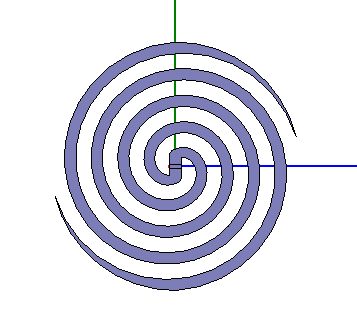
\includegraphics[keepaspectratio, width=110mm]{Images/spiral_antenna_configuration.png}
    \caption{設計したスパイラルアンテナの構造}
    \label{fig:spiral_antenna_configuration}
  \end{figure}

  \begin{figure}[htbp]
    \centering
    \begin{minipage}[b]{0.46\hsize}
      \centering
      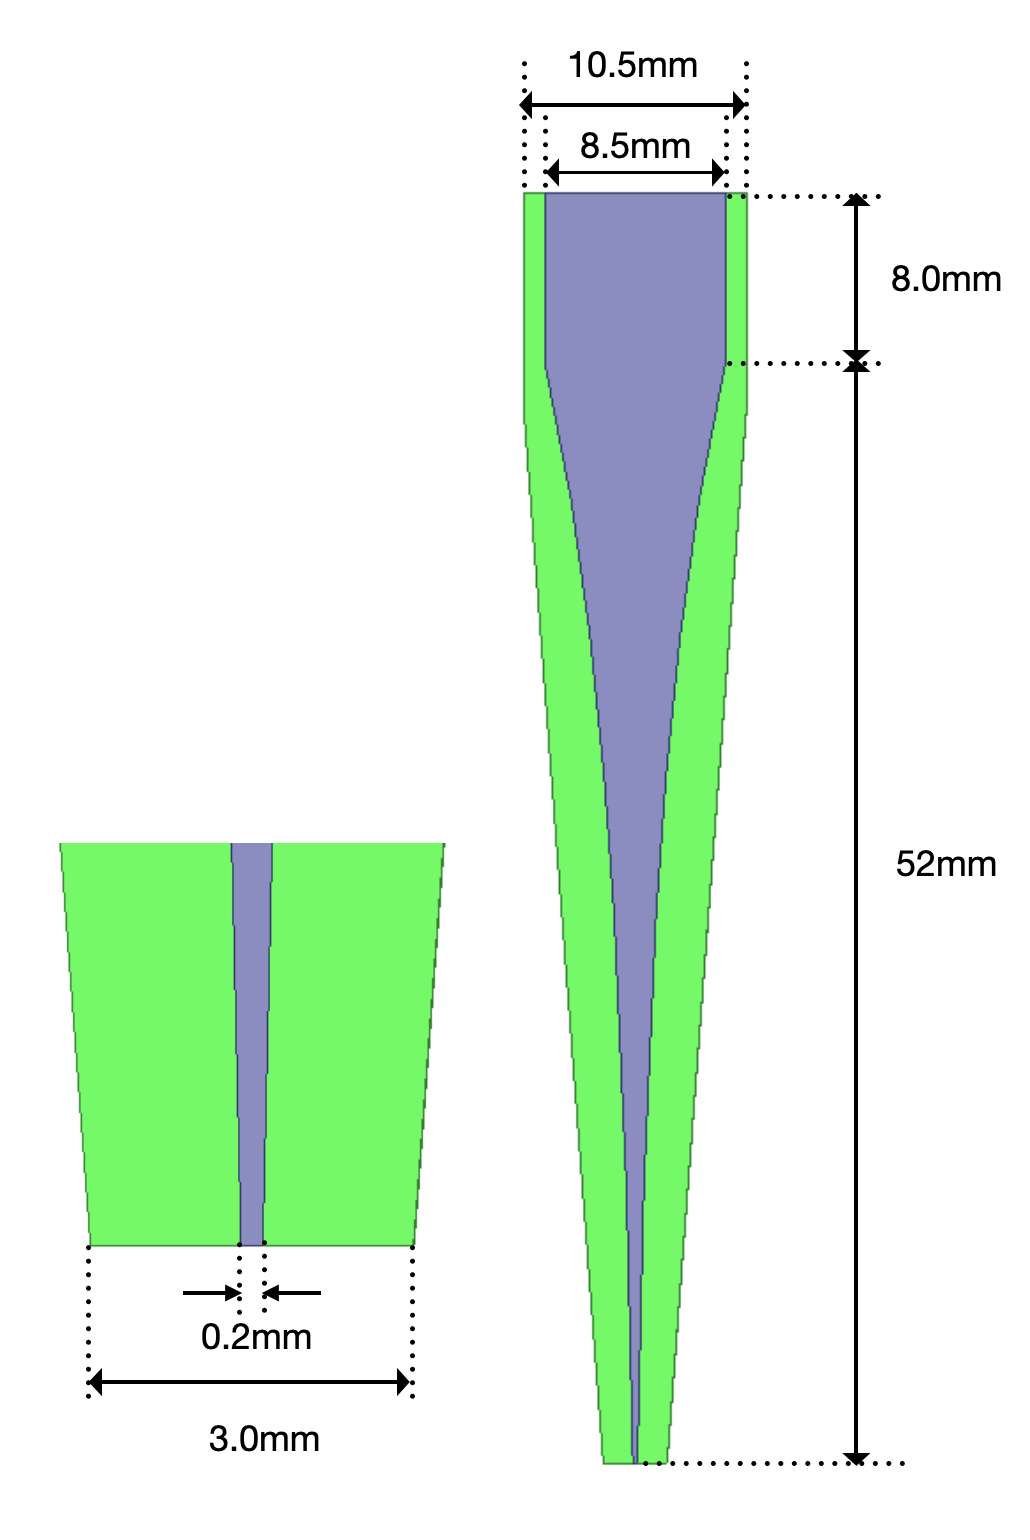
\includegraphics[keepaspectratio, width=75mm]{Images/taper_balun_top.png}
      \subcaption{下面図}
    \end{minipage}
    \begin{minipage}[b]{0.46\hsize}
      \centering
      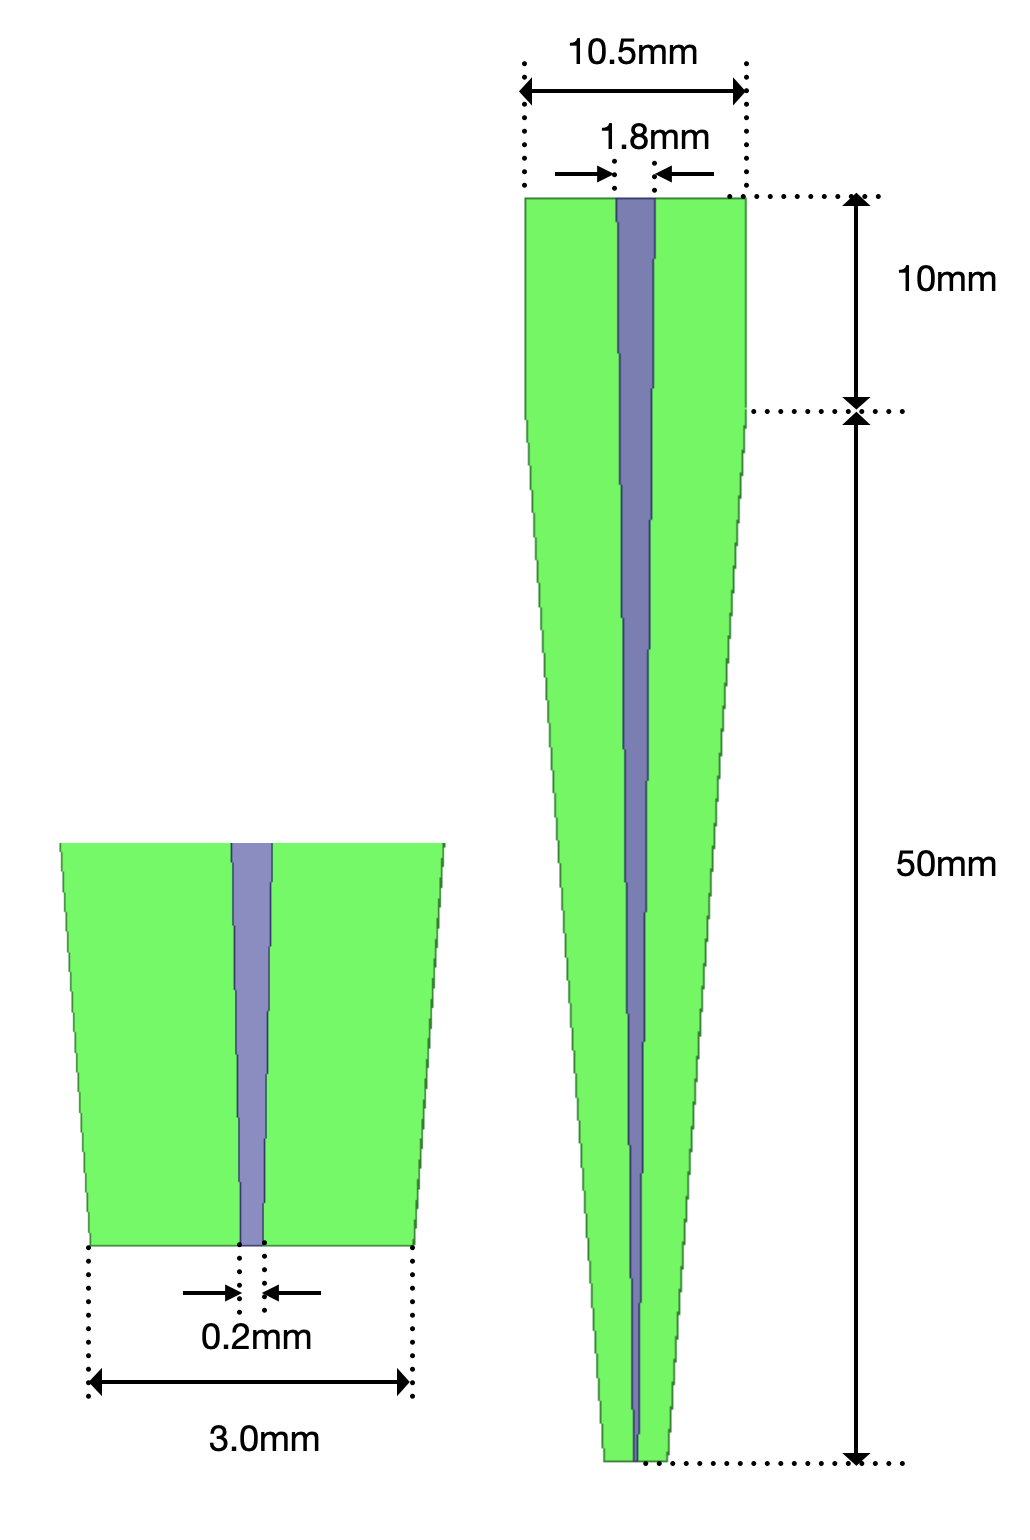
\includegraphics[keepaspectratio, width=75mm]{Images/taper_balun_bottom.png}
      \subcaption{上面図}
    \end{minipage}
    \caption{バランの構造}\label{fig:taper_balun_configuration}
  \end{figure}

  設計したアンテナについて、右円偏波および左円偏波について、5GHz、10GHz、15GHzでゲインをシミュレーションにより計算した2次元にプロットしたものを図\ref{fig:radiation_pattern_2D}
  に示す。また、このうち右円偏波については、5GHz、10GHz、15GHzの角周波数での放射パターンの3次元で可視化したものを図\ref{fig:radiation_pattern_3D}に示す。
  このアンテナは地中レーダに用いるため、所望の偏波状態については、地面に向いている面についてのみ高いゲインを持っていることが望ましい。図\ref{fig:radiation_pattern_2D}
  から、アンテナ面に対して地面と反対側の面についてはゲインが概ね$-10\mathrm{dB_i}$以下と低く抑えられている一方、地面に向ける面の鉛直下向きから$\displaystyle \pm 30^{\circ}$
  程度の範囲についてはゲインが各周波数で$6\mathrm{dB_i}$程度と高く設計できていたことがわかった。

  また、設計したアンテナの軸比の周波数特性のシミュレーションによる計算結果を図\ref{fig:axial_ratio}に示す。
  5GHz - 15GHz にわたって軸比が$<3\mathrm{dB}$、特に5GHz - 7GHzでは軸比が0.5dB以下となっていて、円偏波アンテナとして良好な軸比特性であることが確認できた。

  さらに、設計したアンテナの入力インピーダンスの周波数特性を図\ref{fig:spiral_antenna_impedance}に示す。入力インピーダンスの実部は周波数に対して、
  5GHzから15GHzの範囲で、$190\Omega$程度から$150\Omega$までおよそ線形で減少する特性を示していた。

  テーパバランのマイクロストリップライン部分の設計については、マイクロストリップライン幅は、同軸給電入力部とアンテナ接続部のそれぞれにおいてインピーダンスが整合するよう
  設計するのが望ましい。これらの幅$w$は、誘電体基盤の厚み$h$および基盤の比誘電率$\varepsilon_r$から計算できる\cite{ground_microstrip_line},\cite{pair_microstrip_line}。
  同軸給電部のマイクロストリップライン幅は、その特性インピーダンスが同軸ケーブルの特性インピーダンスと同じ$50\Omega$となるよう、文献\cite{ground_microstrip_line}を参考に計算し
  $w_{\mathrm{in}} = 1.8\mathrm{mm}$とした。アンテナ接続部のマイクロストリップラインについては、アンテナの入力インピーダンスと整合させるためには周波数依存性を持たせるのが望ましいが、
  単純なペアマイクロストリップラインでは特性インピーダンスに周波数依存性を持たせるのが困難であるため、特性インピーダンスが$160\Omega$程度となるよう、文献\cite{pair_microstrip_line}
  を参考に$w_{\mathrm{out}} = 0.2\mathrm{mm}$とした。

  % https://3g-aerial.biz/en/online-calculations/other-calculations/pair-stripline-characteristic-impedance-calculator
  \begin{figure}[htbp]
    \centering
    \begin{minipage}[b]{0.42\hsize}
      \centering
      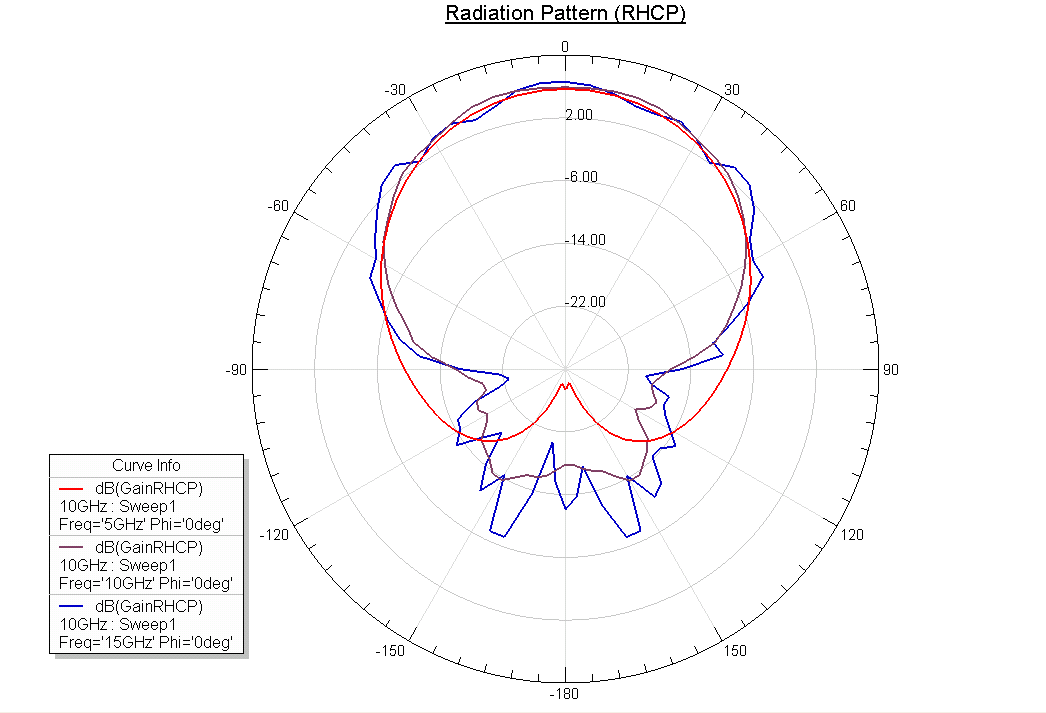
\includegraphics[keepaspectratio, width=80mm]{Images/radiation_pattern_rhcp.png}
      \subcaption{右円偏波}
    \end{minipage}
    \begin{minipage}[b]{0.42\hsize}
      \centering
      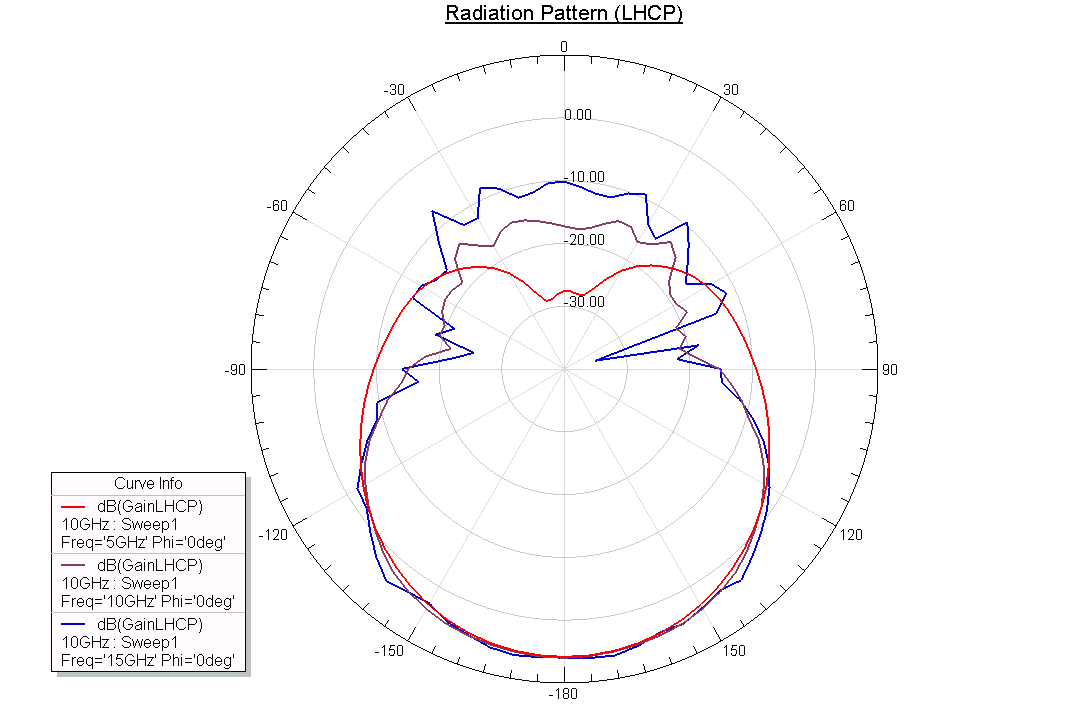
\includegraphics[keepaspectratio, width=80mm]{Images/radiation_pattern_lhcp.png}
      \subcaption{左円偏波}
    \end{minipage}
    \caption{放射パターンの2次元プロット}\label{fig:radiation_pattern_2D}
  \end{figure}

  \begin{figure}[htbp]
    \centering
    \begin{minipage}[b]{0.45\hsize}
      \centering
      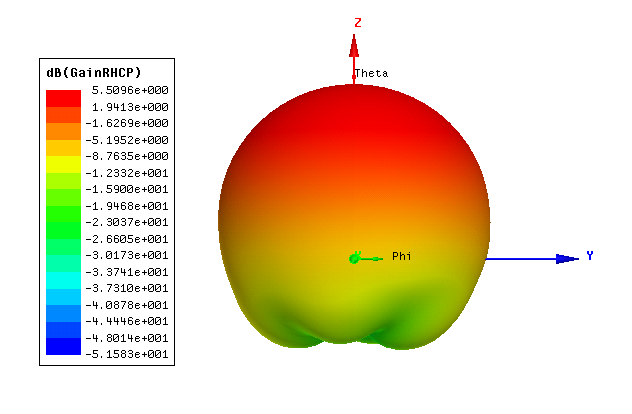
\includegraphics[keepaspectratio, width=80mm]{Images/gain_rhcp_5GHz.png}
      \subcaption{5GHz}
    \end{minipage}
    \begin{minipage}[b]{0.45\hsize}
      \centering
      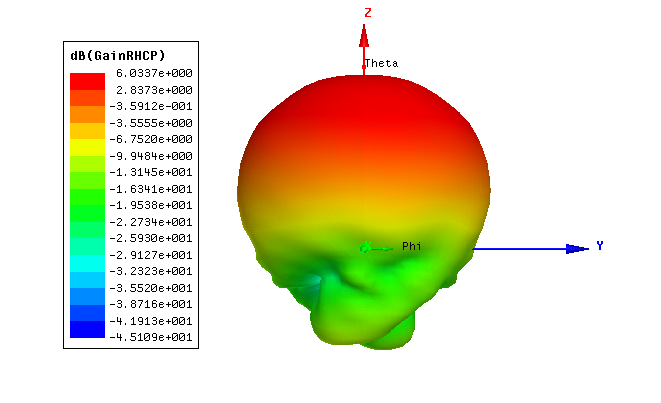
\includegraphics[keepaspectratio, width=80mm]{Images/gain_rhcp_10GHz.png}
      \subcaption{10GHz}
    \end{minipage}
    \begin{minipage}[b]{0.45\hsize}
      \centering
      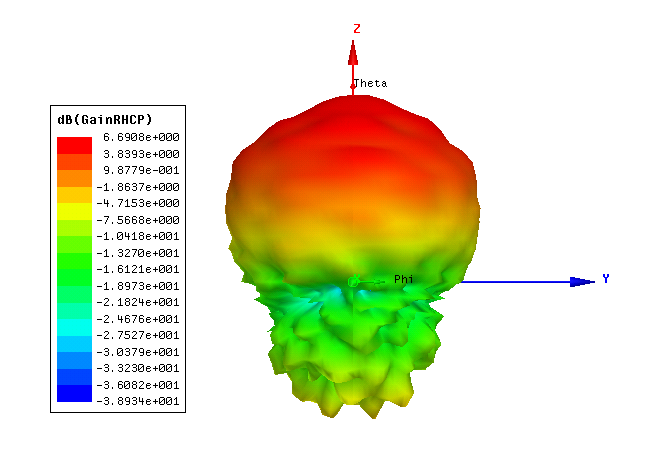
\includegraphics[keepaspectratio, width=80mm]{Images/gain_rhcp_15GHz.png}
      \subcaption{15GHz}
    \end{minipage}
    \caption{放射パターンの3次元プロット}\label{fig:radiation_pattern_3D}
  \end{figure}

  \begin{figure}[hbtp]
    \centering
    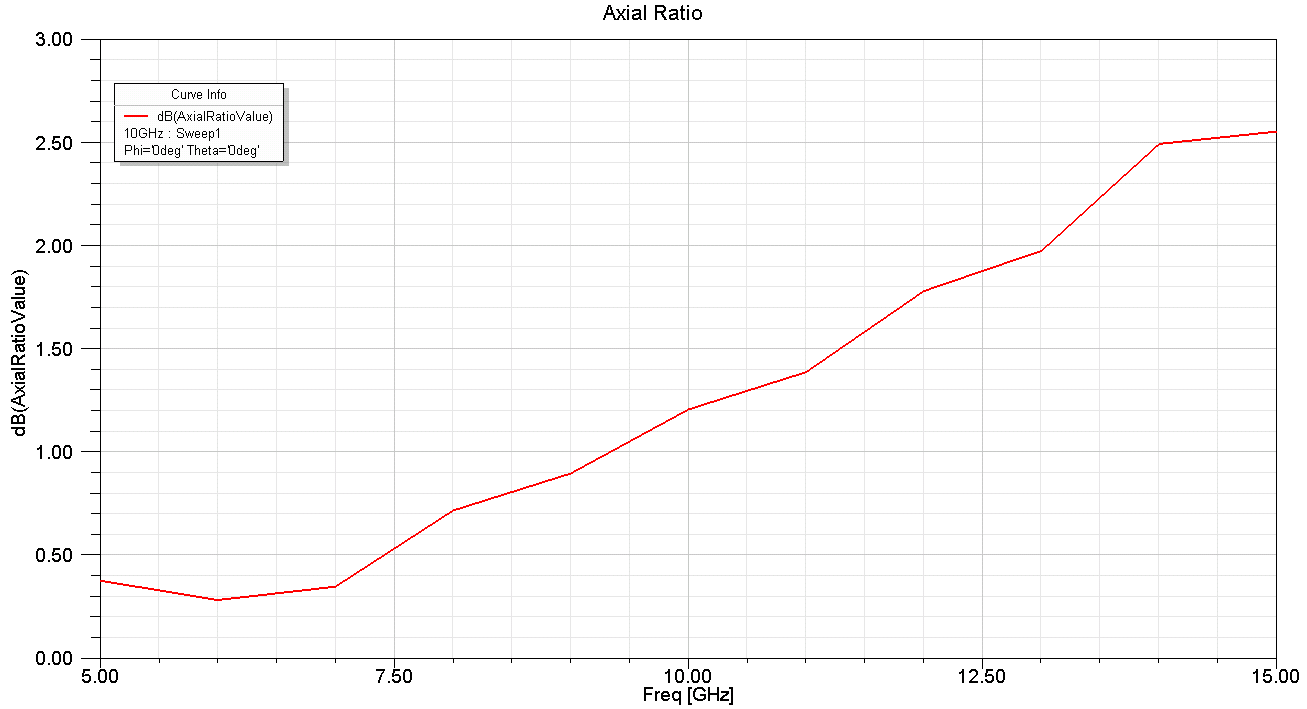
\includegraphics[keepaspectratio, width=130mm]{Images/axial_ratio.png}
    \caption{設計したアンテナにおける軸比の周波数特性}
    \label{fig:axial_ratio}
  \end{figure}

  \begin{figure}[hbtp]
    \centering
    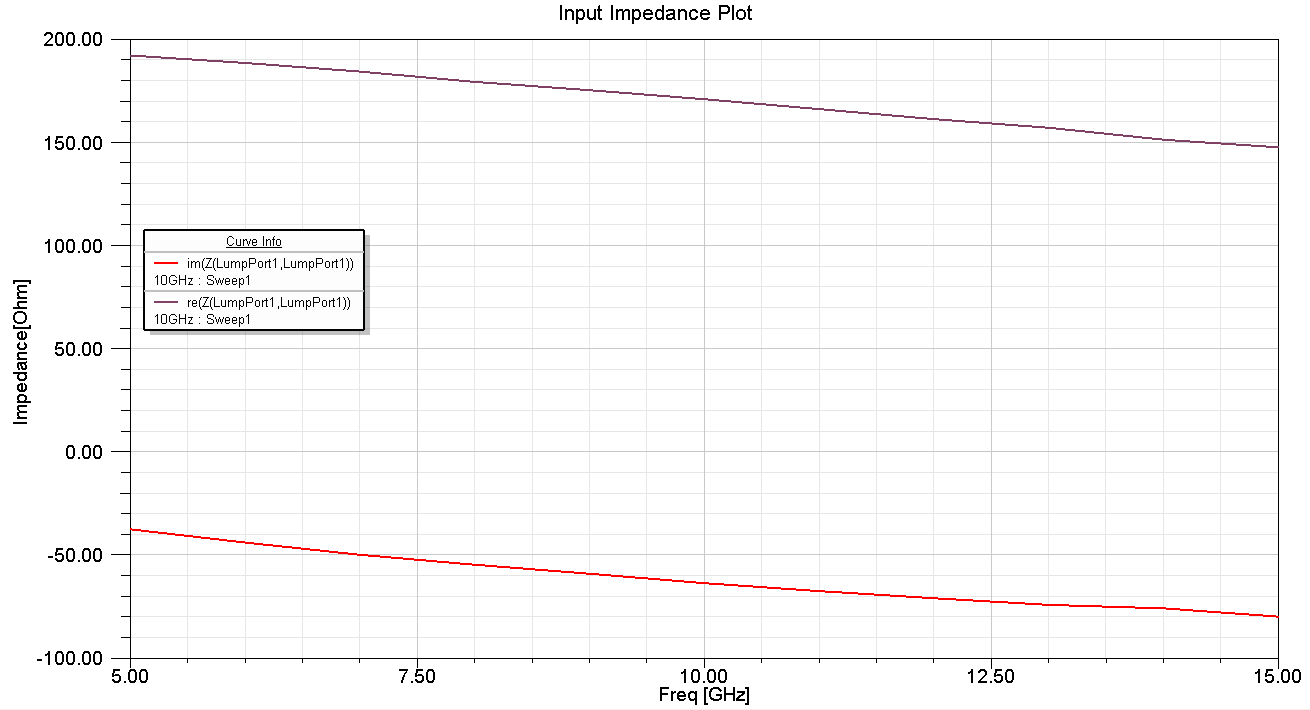
\includegraphics[keepaspectratio, width=130mm]{Images/spiral_impedance.png}
    \caption{設計したアンテナにおける入力インピーダンスの周波数特性}
    \label{fig:spiral_antenna_impedance}
  \end{figure}

\newpage

  \subsection{地中レーダシステムによる計測}
  複素ニューラルネットワークの学習及び検証に用いるデータは、先述の計測システムを用いて取得する。計測対象としては、
  図\ref{}に示すような、長さ150mm、外径27mmの中空鉄パイプ管を用いた。このパイプ管を、地中40mmの深さに埋設した。

  このようにしてパイプ管を埋設した砂槽に対して、図\ref{}に示すように、10mm間隔の35×35の測定点に対して測定を行った。
  各測定点において、周波数を1.00Ghzから11.00GHzまで0.05Ghzごとの201点で掃引した電磁波を円偏波アンテナを用いて放射し、受信アンテナにおける
  受信信号を伝送係数$S_{21}$として計測した。これを一回の計測として、各受信アンテナの方向H, V、および、パイプの向きを
  図\ref{}%TODO: パイプの向きの図を挿入
  のように$0^{\circ}$から$170^{\circ}$まで$10^{\circ}$刻みで変えた計36回の計測を行った。

  なお、図\ref{}に示すように、H方向の受信アンテナとV方向の受信アンテナは、円偏波送信アンテナにたいしてずれた位置に配置されているため、
  送受信アンテナの中点が動く範囲がHおよびV方向の受信アンテナで同じ範囲になるよう、図\ref{}に示すように、
  測定の開始点はH方向およびV方向で異なる位置に設定した。

  % \begin{table}[h]
  %   \centering
  %   \caption{実験条件のまとめ}
  %   \begin{tabular}{|c|c|c|} % 列の数や形式に応じて調整してください
  %     \hline
  %     実験条件 & パラメータ1 & パラメータ2 \\
  %     \hline
  %     条件1 & 値1 & 値2 \\
  %     条件2 & 値3 & 値4 \\
  %     % 必要なだけ行を追加
  %     \hline
  %   \end{tabular}
  % \end{table}

  %写真を貼る 鉄パイプ
  \subsection{複素ニューラルネットワークを用いた解析}
  地中レーダシステムによって得られたデータを、複素ニューラルネットワークを用いて解析した。ここでは、まず入力データの形式について述べ、
  その後に複素ニューラルネットワークの構成について述べる。
  \subsubsection{入力データの形式}
  本実験では、35×35の測定点に対し$S_{21}^{H}$をそのまま入力データとして用いるパターンと、H受信とV受信の間の伝送係数の比をとった
  $\cfrac{S_{21}^{H}}{S_{21}^{V}}$を入力データとして用いるパターンの2通りについて実験を行った。

  まず、それを5点おきにサンプリングした7×7のデータを用意した。1つのサンプリングされたデータに対し、データセットの拡張のために、
  これらを0°、90°、180°、270°回転させ、さらにそれぞれについて画像を反転させたデータを用意した。
  これにより、1回の測定当たり25 * 4 * 2 = 200個のデータを得ることができる。したがって、データセットのサイズは、18 * 200 = 3600 個となる。
  このうち、2700個を学習データとし、残り900個をテストデータとした。

  
  \subsubsection{入力データの形式}
  本実験では、畳み込み層を1層、全結合層を1層とした複素ニューラルネットワークを用いた。
  畳み込み層の層数は16とし、活性化関数には複素tanh関数を用いた。また、学習率については のようにした。
  教師データの与え方としては、次の3通りについて実験を行った。
  \[
    \mathbf{v}_j =
    \begin{cases}
        1 & \text{if } j = i, \\
        0 & \text{otherwise}.
    \end{cases}
  \]
  \[
    \mathbf{v}_j =
    \begin{cases}
        1 & \text{if } j = i, \\
        0 & \text{if} j = i \pm 1 \text{or} {i, j} = {0, 17}.\\
        -1 & \text{otherwise}.
    \end{cases}
  \]
  \[
    \mathbf{v}_j = e^{i\cdot2\theta}
  \]
  ここで、$\mathbf{v}_j$は教師データの$j$番目の要素を表し、$i$は、対象物の角度が0°の場合のクラスを0、10°の場合のクラスを1、...、170°の場合のクラスを17としたときの
  クラスの番号を表す。また、$\theta$は対象物の向きをラジアン表記したものを表す。
  1つ目の教師データの与え方は、対象物の向きをクラス分けしたものを教師データとして与えるものである。クラスの番号に一致する要素には1を、それ以外の要素には0を与える。
  2つ目の教師データの与え方は、クラス間の類似度に関して、角度が$\pm10^{\circ}$異なるクラス
  を正解に近いクラスとして評価し、クラスの番号に一致する要素には1を、 角度が$\pm10^{\circ}$異なるクラスの番号には0を、それ以外の要素には-1を与えるものである。
  3つ目の教師データの与え方は、対象物の角度推定を、分類問題ではなく、角度を数値として予測する回帰問題としてとらえ、対象物の向きを複素数として与えるものである。
  パイプの向きは$\pm180^{\circ} = \pi$周期の周期性があるため、$\pi$の周期性を持つ複素数として$e^{i\cdot2\theta}$を与えている。

  ここで、1つ目および2つ目の教師データの与え方については、最終的な出力のニューロン数が18、3つ目の教師データの与え方の場合には、最終的な出力のニューロン数が1
  となっている。これらの各ニューロンは、直前の畳み込み層の出力から、全結合層を経て出力される。すなわち、最終層の$i$番目のニューロンの出力$y_i$は、
  \[
    \mathbf{v}_i = f(\sum_{j=1}^{16} \sum_{k=1}^{16} \mathbf{w}_{ijk} \cdot \mathbf{z}_{jk} + \mathbf{b}_i)
  \]
  となる。(TODO: 改善)
  学習の最適化には、SGDを用いた。(TODO: 引用)学習率は0.001、ミニバッチサイズは32、エポック数は20とした。学習の進行度は、誤差関数として用いている
  平均二乗誤差に加え、分類型の教師データの場合には正解率を、回帰型の教師データに対しては位相差を用いて評価した。
  正解率は、次式で定義する。
  \[
    \text{正解率} = \frac{n(\{x \in S \, |\, class(x) = \})}{n(S)}
  \] %TODO: 修正
  \[
    \text{位相差} = \frac{n(\{x \in S \, |\, class(x) = \})}{n(S)}
  \] %TODO: 修正
  を用いて評価した。

\section{結果}
  各条件における、誤差関数の値の推移を図\ref{}に示す。
  
  
\section{考察}
  

\section{今後の展望}

  \subsection{計測システムの構築}

    アンテナやバラン部分については、Ansys HFSSを用いた設計自体は行ったが、実際に基盤加工器などを用いた部品の作成は未完了である。まずはこれを完了させ、
    実際に計測システムが動作することを確認したい。計測対象としては鉄パイプ管を用い、その深さや向きを様々に変えてデータ収集を行うことを想定している。

  \subsection{複素ニューラルネットワークを用いた解析システムの構築}\label{CVNN_plan}

    本研究は、複素ニューラルネットワークを用いて、円偏波地中レーダシステムにより取得したデータから、対象物の向きや形状などの幾何構造や、
    対象物の存在する座標などの特徴量を抽出することを目標としている。本実験では鉄パイプ管を用いるため、特徴量としてパイプの深さや向きを出力できるような
    複素ニューラルネットワークシステムの構築を模索する予定である。システムの構築に際して考慮すべき点としては、教師データの与え方、入力データの形式、
    隠れ層の層数や各層のニューロン数、学習方法や学習におけるパラメータなどがあると考えられる。これらを適切に設定し、より高精度なシステムを構築したいと考えている。


\bibliographystyle{ieeetr}
\bibliography{refs}

\end{document}